% !TEX root = thesis.tex
\startchapter{Communication and Failure}
\label{chap:soc-net}
We open our investigation of how to modify the social relationships among software developers, represented by the communication between them, with searching for a relationship between communication and build success.
This will form the basis and justification for an approach that we will describe in a later chapter to allow us to manipulate the social interactions among developers.
Thus this chapter explores our first research question
\begin{description}
\item[RQ 1.1] Do Social Networks from repositories influence build success?
\end{description}

A connection between communication among developer and any sort of software quality including software builds makes intuitively sense.
For example, any non trivial software project consists of several interdependent modules and with the growing size and number of modules the work of more than one software developer is required to finish the project within a certain time constraint often mandated by a customer.
Now due to the interdependence of the software modules developer assigned either to the same or to interdependent module need to coordinate their work.
This coordination is in the most part accomplished through communication, which can take any form from a face-to-face discussion to electronically asynchronous messages such as email.
Coupled with the fact that communication is inherently ambiguous and can often lead to misunderstandings, errors based on such misunderstandings may be introduces into the source code.
Thus, we are confident that there exists  a connection between developer communication and build success.

In the remainder of this chapter, we start with detailing the back ground relevant to studying communication in relationship to software builds or to integration issues in software development in a broader sense (Section~\ref{ch5:bg}).
Subsequently, we describe the methodology that is relevant to exploring our research question (Section~\ref{sec:Methodology}).
Then, we present our the analysis and results we obtained in Section~\ref{sec:AnalysisResults} followed by a discussion of the results and their implications in Section~\ref{sec:discussion}.
We conclude this chapter with offering an answer to our research question and leading into the subsequent Chapter~\ref{chap:stc-net2} (Section~\ref{sec:conclusion}).


\section{Background}
\label{ch5:bg}
Before we start exploring the research question using data we obtained from the Rational Team Concert Team, we discuss related work investigating the relationship between team communication with respect to software integration issues as well as software quality and thus further motivating the value in investigating the relationship between communication and build success.

\subsection{Motivation}
Communication problems can lead to coordination and integration failures in work
teams (e.g.~\cite{Grinter:1999geography,Herbsleb:1999ew,souza:cscw:2004}). This
situation is further exacerbated in large and distributed teams, where effective
communication and activity awareness of related but remote project members are
problematic, yet key to anticipate and resolve coordination problems early
(e.g.~\cite{Grinter:1999geography,Herbsleb:1999ew}).

We strive to contribute to the growing body of research into the role of
communication structures in determining coordination ease~\cite{hinds:cscw:2006} and
success~\cite{hossain:cscw:2006}. Although there has been some research on the
relationship between communication and coordination in work teams, research in
software engineering is very limited. The study of the Enron email corpus found
that central communicators exhibit a better ability to
coordinate~\cite{hossain:cscw:2006} and R\&D teams with dense communication
structures are associated with more coordination problems~\cite{hinds:cscw:2006}. In
open source software development, developers that are active in email
communication have also been found to be most active in open source
development~\cite{bird:msr:2006}. In software engineering research, however it is
unclear whether there are specific communication behaviors that enable effective
coordination. Moreover, we are missing a precise conceptualization and objective
measure of what successful communication in relation to project success is.

Complementary to previous research that is largely qualitative
\cite{herbsleb2003:speed,Holmstrom:2006gd} and which gathered information about
occurrences of communication problems through project reviews and subjective
ratings of project success, we use objective measures in studying the
relationship between communication structures and coordination success. Past
research has also largely investigated communication and coordination only in
relation to entire projects. There is little systematic software engineering
research in objectively examining the outcome of coordination (successful or
failed) and assessing communication characteristics that lead to coordination
failures. In this work we investigate the relationship between communication
structures and coordination outcome at a finer level of detail. We study
instances of coordination during the integration of code in large and distributed
software teams, in relation to their associated communication structures. By
communication structure we refer to the topology of the communication network
that was involved in the tasks that lead to a software build. We use social
network analysis measures such as density and centrality to obtain measurable
characteristics of the communication structure.


\subsection{Communication, Coordination and Integration}
\label{sec:RelatedCommunication}
The relationship between communication, coordination and project outcome has been
studied for a long time in the area of computer-supported cooperative work. More
recently the domain of software and distributed software development showed
increased interest as well.

Communication plays an important role in work groups with high coordination needs
and the quality of communication has been found as determinant of project
success~\cite{curtis:acm:1988,kraut:1995coordination}. The dynamic nature
of work dependencies in software development makes collaboration highly
volatile~\cite{Cataldo:2007hb}, consequently affecting a teams ability to
effectively communicate and coordinate. Additional difficulties emerge in
distributed teams, where team membership and work dependencies become even more
invisible~\cite{damian:icgse:2007}. Moreover, team communication patterns are
significantly affected by distance~\cite{hinds:cscw:2006}. Maintaining
awareness~\cite{sarma:2006icgse} becomes even more difficult when developers work
in geographically remote environments; communication structures that include key
contact people at each site are effective coordination strategies when
maintaining personal cross-site relationships is challenging~\cite{hinds:cscw:2006}.

With respect to the role of effective coordination in project success, early
studies indicate the issues that software development teams face in large
projects~\cite{curtis:acm:1988}. A study by Herbsleb et
al.~\cite{Herbsleb:1999ew} showed that Conway's law is also applicable for the
coordination within development teams, supporting the influence of coordination
on software projects. Kraut et al.~\cite{kraut:1995coordination} showed that
software projects are greatly influenced by the quality of coordination of
development teams. More recently a theory of coordination has been proposed and
accounts for the influence of coordination on different project metrics such as
rework and defects~\cite{Herbsleb:2006vn}.


The importance of communication in successful coordination is also well
documented and makes the study of communication structures important. For
example, Fussell et al.~\cite{fussell:cscw:1998} found that communication amount and
tactics were linked to the ability of effectively coordinate in work groups. In
software development, others showed that communication problems lead to problems
during the activity of subsystem
integration~\cite{Grinter:1999geography,deSouza2004:thwarts_collaboration}. Coordination
conceptualized via communication has also been studied more generally in relation
to project success: factors such as ``harmony''~\cite{Souder:1988jpim},
communication structure~\cite{Robin:1990jpim}, and communication
frequency~\cite{Griffin:1992ms} were related to project success.

The difficulty in studying failed integration in relation to communication lies
in capturing and quantifying information about communication in teams that have a
well-defined coordination goal but dynamic patterns of interaction. In our work
we use the Jazz project data, which captures communication of project
participants. This enables us to study the structure of the communication
networks emerged around code integrations, both at individual teams of the
project and within the entire project.

\subsection{Can communication predict failure?}
\label{sec:ResearchQuestions}
In order to examine the communication involved in the coordination necessary
during subsystem integrations, we draw on social network analysis methods. Social
network analysis has often been deployed to study communication networks of work
teams. Using social network analysis has the major advantage that we can draw
from its extensive knowledge of analysis and implications with respect to social,
communication, and knowledge management
processes~\cite{Burt:1995vo,Freeman:1979rl}. Griffin and
Hauser~\cite{Griffin:1992ms} investigated social networks in manufacturing teams.
They found that a higher connectivity between engineering and marketing increases
the likelihood of a successful product. Similarly, Reagans and
Zuckerman~\cite{RayReagans:2001os} related higher perceived outcomes to denser
communication networks in a study of research and development teams.

Communication structure in particular -- the topology of a communication network
-- has been studied in relation to coordination
(e.g.~\cite{hossain:cscw:2006,hinds:cscw:2006}) and a number of common measures of
communication structure include network density, centrality and structural
holes~\cite{Wasserman:1994sq,Freeman:1979rl}.

Density, as a measure of the extent to which all members in a team are
connected to one another, reflects the ability to distribute
knowledge~\cite{Rulke:2000ys}. Density has been studied, for example, in relation
to coordination ease~\cite{hinds:cscw:2006}, coordination
capability~\cite{hossain:cscw:2006} and enhanced group
identification~\cite{RayReagans:2001os}.


Centrality measures indicate importance or prominence of actors in a
social network. The most commonly used centrality measures include degree and
betweenness centrality having different social implication. Centrality measures
have been used to characterize and compare different communication networks
constructed from email correspondence of W3C (WWW consortium) collaborating
working groups developing new technical standards and architectures for the
web~\cite{Gloor:2003cikm}. Similarly, Hossain et al.~\cite{hossain:cscw:2006}
explored the correlation between centrality in email-based communication networks
and coordination, and found betweenness to be the best measure for coordination.
\emph{Betweenness} is a measure of the extent to which a team member is
positioned on the shortest path in between other two members. People in between
are considered to be ``actors in the middle'' and to have more ``interpersonal
influence'' in the
network(e.g.~\cite{Gloor:2003cikm,zimmermann:icse:2008,hossain:cscw:2006}).

The structural holes measures are concerned with the degree to which there
are missing links in between nodes and with the notion of redundancy in
networks~\cite{Burt:1995vo}. At the node level, structural holes are gaps between
nodes in a social network. At the network level, people on either side of the
hole have access to different flows of information~\cite{Hargadon:1997asq},
indicating that there is a diversity of information flow in the network.
Structural holes have been used to measure social capital in relation to the
performance of academic collaborators (e.g.~\cite{Brambila:PICMET2007}).

To further our investigation into the role played by communication in
predicting integration failure, we go one step further and investigate whether
the different communication structure measures can be combined into a prediction
model that indicates whether an integration will fail.

Past research on failure prediction was not able to find a single code or code
churn metric predicting
failures~\cite{nagappan:icse:2006,basili:1996tse,denaro:2002seke}, though the
combination of those measurements became a strong predictor
(e.g.~\cite{mockus:2000bell}). This leads us to believe that even if we do not
find a single communication structure measure that predicts integration outcome,
it is useful to combine the communication network measures -- as a reflection of
the communication structure of a team -- into a predictive model and study its
predictive power.

Most prediction models in software engineering to date mainly leverage source
code related data and focus on predicting failing software components or failure
inducing changes
(e.g.~\cite{bell:2005tse,schroeter:isese:2006,zimmermann:icse:2008,kim:2008tse}).
Only few studies, such as Hassan and Zhang~\cite{hassan:ase:2006}, stepped away
from predicting component failures and used statistical classifiers to predict
integration outcome. Recently, we can observe a trend towards leveraging
developer networks, created upon code related dependencies, to predict component
failures~\cite{pinzger:fse:2008,meneely:fse:2008}. In our work, we focus on the
team coordination as given by their communication instead of source code, and
similar to Hassan and Zhang predict integration outcome.


\section{Methodology}
\label{sec:Methodology}

To address our research questions we analyze data from a large software
development project, IBM's Jazz~\cite{frost:ieeesoftware:2007}. With collaboration support
as one of its main goals, Jazz provides integrated support for work planning and
tracking, communication and collaboration, and continuous integration builds. For
our research, Jazz provides the traceability between communication artifacts and
development artifacts, important in the study of coordination processes. In what
follows we first describe in detail the coordination and integration process in
Jazz as the context for our investigation. We then explain how we conceptualized
communication and integration outcome in Jazz, as well as the data collection
instruments.

\subsection{Coordination outcome measure}
In our study we conceptualize the coordination outcome by the \et{Build Result},
which is regarded as a coordination success indicator in Jazz and can be \error,
\texttt{WARNING} or \ok. We analyze build results to examine the integration
outcomes in relation to the communication necessary for the coordination of the
build.

Conceptually, the \texttt{WARNING} and \ok\ build results are treated similar by
the Jazz team, as they require no further attention or reaction from the
developers. In contrast, \error\ build results indicate serious problems such as
compile errors or test failures and require further coordination, communication
and development effort. We thus treated all \texttt{WARNING}s as \ok s to clearly
separate between failed and successful builds in our conceptualization of
coordination outcome.


\subsection{Communication network measures}
To characterize the communication structure represented by the constructed social
networks for each build (as described in Chapter~\ref{chap:meth}), we compute a number of social network measures. The
measures that we include in our analysis are: Density, Centrality and Structural
holes. Some of these measures characterize single nodes and their neighbours (ego
networks), while others relate to complete networks. As we are interested in
analysing the characteristics of complete communication networks associated to
integration builds, we normalize and use appropriate formulas to measure the
complete communication networks instead of measuring the individual nodes.

\subsubsection{Density}
Density is calculated as the percentage of the existing connections to all
possible connections in the network. A fully connected network has a density of
1, while a network without any connections has the density of 0. For example, the
density in the directed network in Figure~\ref{fig:CentralityExample} is
$12/42=0.28$.

\subsubsection{Centrality measures}
We use the centrality measures \emph{group degree centralization} and
\emph{group betweenness centralization} for complete networks, which are based on
the ego network measures degree centrality and betweenness. The degree
centrality measures for the ego networks are:

\begin{itemize}
  \item The \emph{Out-Degree} of a node $c$ is the
  number of its outgoing connections $C_{oD}(c)$. E.g. $C_{oD}(c_1)=2$ in 
  Figure~\ref{fig:CentralityExample}.
  
  \item The \emph{In-Degree} of a node $c$ is the
  number of it s incoming connections $C_{iD}(c)$. E.g.$C_{iD}(c_1)=1$ 
  in Figure~\ref{fig:CentralityExample}.
  
  \item The \emph{InOut-Degree} of a node $c$ is the sum of its In-Degree and
  Out-Degree $C_{ioD}(c)$. E.g. $C_{ioD}(c_1)=3$
  in Figure~\ref{fig:CentralityExample}.
\end{itemize}

To compute the \emph{Group Degree Centralization} index for the complete network
we use formula~(\ref{eq:GroupDegreeCentralization}) from
Freeman~\cite{Freeman:1979rl}, in which $g$ is the number of nodes in a network,
and $C_D(c_i)$ is any of the degree centrality measures of a node $c_i$ as
described above. $C_D(c^*)$ is the largest node degree index for the set of
contributors in the network. The formula is also used
by~\cite{Gloor:2003cikm,hinds:cscw:2006}.

\begin{equation}
\displaystyle C_D =  \frac{\sum_{i=1}^g[C_D(c^*) - C_D(c_i)]}{(g-1)^2}
\label{eq:GroupDegreeCentralization}
\end{equation}

\begin{figure}[t]
\begin{center}
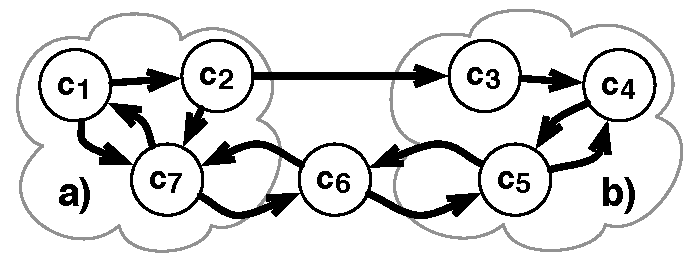
\includegraphics[width=.4\columnwidth]{figures/CentralityExample}
\caption{Example of a directed network to illustrate our social
analysis measures.}
\label{fig:CentralityExample}
\end{center}
\end{figure}

To calculate the \emph{Group Betweenness Centralization} index for a whole
network, we need to compute the betweenness centrality probability index for each
actor of the network. The probability index assumes that a ``communication''
takes the shortest path from a contributor $c_j$ to contributor $c_k$ and if the
network has more shortest paths, all of them have the same probability to be
chosen. If $g_{jk}$ is the number of shortest paths linking two contributors,
$1/g_{jk}$ is the probability of using one of the shortest paths for
communication. Let $g_{jk}(c_i)$ be the number of shortest paths linking two
contributors that contain the contributors $c_i$. Freeman~\cite{Freeman:1979rl}
estimates the probability that contributor $c_i$ is between $c_j$ and $c_k$ by
$g_{jk}(c_1)/g_{jk}$. The betweenness index for $c_i$ is the sum of all
probabilities over all pairs of actors excluding the $i$th contributor.
Formula~(\ref{eq:Betweenness}) shows the normalized betweenness index for
directed networks.

\begin{equation}
\displaystyle C_B(c_i) =  \frac{\sum_{j<k} g_{jk}(c_i)/g_{jk}}{(g-1)(g-2)}
\label{eq:Betweenness}
\end{equation}

To compute a betweenness index for the complete network instead of a single node,
we used Freeman's formula for \emph{Group Betweenness Centralization}. The
formula is shown in equation~(\ref{eq:GroupBetweenness}), in which $C_B(c^*)$ is
the largest betweenness index of all actors in the network.

\begin{equation}
\displaystyle C_B =  \frac{\sum_{i=1}^g[C_B(c^*)-C_B(c_i)]}{(g-1)}
\label{eq:GroupBetweenness}
\end{equation}


\subsubsection{Structural holes}
We use the following structural hole measures:
\begin{itemize}
  \item The \emph{Effective Size} of a node $c_i$ is the number of its
  neighbours minus the average degree of those in $c_i$'s ego network, not
  counting their connections to $c_i$. The effective size of node $c_1$ in 
  Figure~\ref{fig:CentralityExample}a is $2-1=1$. Note, that only direct
  neighbours of $c_1$ are considered and the directed connections are replace
  with undirected. The effective size of node $c_4$ in 
  Figure~\ref{fig:CentralityExample}b is $2-0=2$.
  
  \item The \emph{Efficiency} normalizes the effective size of a node $c_i$ by
  dividing the it's effective size with the number of it's neighbours. The
  efficiency of node $c_1$ in Figure~\ref{fig:CentralityExample}a is
  $(2-1)/2=0.5$. The efficiency of node $c_4$ in
  Figure~\ref{fig:CentralityExample}b is $(2-0)/2=1$.
  
  \item \emph{Constraint} is a summary measure that relates the connections of a
  node $c_i$ to the connections of $c_i$'s neighbours. If $c_i$'s neighbours and
  potential communication partners all have one another as potential communication
  partners, $c_i$ is highly constrained. If $c_i$'s neighbours do not have other
  alternatives in the neighborhood, they cannot constrain $c_i$'s behavior. 
\end{itemize}

To calculate network measures of the introduced ego network measures on
structural holes, we compute the sum of the measures for each node of a network.
As the measures are based on network connections, we normalize the sum by
computing the fraction of the sum and the number of possible network connections.

\subsection{Data collection} 
We mined the Jazz development repository for build and communication information.
A query plug-in was implemented to extract all development and communication
artifacts involved in each build from the Jazz server. These build-related
artifacts included build results, teams, change sets, work items, contributors,
and comments. We imported the resulting data into a relational database
management system to handle the data more efficiently.

We extracted a total of 1288 build results, 13020 change sets, 25713 work item
and 71019 comments. Out of a total of 47 Jazz teams, 24 had integration builds.
The build results we extracted were created during the time range from
November~5, 2007 to February~26, 2008.

Next, we had to make a decision for which builds and associated communication to
analyze. Our selection criteria was that we analyze a number of build results
that is large enough for statistical tests and include both \ok\ and \error\
builds. Some teams used the building process for testing puroses only and created
just a view build results, while others had either only \ok\ or only \error\
build results. Predicting build results for a team that only produced \error\
builds in the past, will most likely yield an \error, since no communication
information representing successful builds is available. Thus, we considered
teams that had more than 30 build results and at least 10 failed and 10
successful builds. Five teams satisfied these constraints and were considered in
our analysis. In addition, we included the nightly, weekly, and one beta
integration build, although they did not satisfy our constraints, because 
they integrate all subsystems of the entire project.






\section{Analysis and Results}
\label{sec:AnalysisResults}
% In this section we describe our analysis techniques for our research questions.
Table~\ref{tab:DescriptiveStats} shows descriptive statistics of the considered
builds and related communication networks of the five teams (B, C, F, P and W in
the first 5 columns) and the nightly, weekly, and beta project-level
integrations. For example, team B created 60 builds from which 20 turned out to
be \error s and 40 \ok. The communication networks of this team had between 3 and
58 contributors (51.58 directed connections in average) and spanned 0 to 131 work
items. The builds involved in average 10.83 change sets.

\begin{table}[t]
\footnotesize
\begin{center}
%{\small
\begin{tabular}{r@{\hspace{15pt}}c@{\hspace{5pt}}c@{\hspace{5pt}}c@{\hspace{5pt}}c@{\hspace{5pt}}c@{\hspace{15pt}}c@{\hspace{5pt}}c@{\hspace{5pt}}c}
\toprule
%  & & & Teams & & & & & &  \\
& \multicolumn{5}{ c@{\hspace{3pt}}}{Team Level Builds} &
\multicolumn{3}{c}{Project Level Builds} \\ & B & C & F & P & W & nightly &
weekly & beta
\\
\midrule
\# Builds & 60 & 48 & 55 & 59 & 55 & 15 & 15 & 16 \\ 
\# \error s & 20 & 16 & 24 & 29 & 31 & 9 & 11 & 13 \\ 
\# \ok s & 40 & 32 & 31 & 30 & 24 & 6 & 4 & 3 \\ 
%First Build & 2007-11-05 14:04:48 & 2007-11-09 07:22:05 & 2007-11-06 03:36:48
%& 2007-11-05 22:28:45 & 2007-11-09 17:01:35 & 2007-11-05 03:59:06 & 2007-07-24
%21:19:07 & 2007-12-04 14:23:20 \\ 
%Last Build & 2008-02-26 15:43:59 &
%2008-02-26 13:38:49 & 2008-02-22 16:34:25 & 2008-02-26 11:43:36 & 2008-02-26
%08:53:04 & 2008-01-18 07:41:26 & 2008-02-22 15:29:39 & 2008-01-23 19:22:41 \\
\midrule
\multicolumn{3}{l}{\emph{\# Contributors:}} \\
%\midrule
Min & 3 & 9 & 6 & 5 & 13 & 43 & 37 & 55 \\ 
Median & 6 & 16.5 & 18 & 15 & 20 & 55 & 57 & 69.5 \\ 
Mean & 12.68 & 18.02 & 20.15 & 17.98 & 22.87 & 57.93 & 52.27 & 67.81 \\ 
Max & 58 & 31 & 64 & 61 & 52 & 75 & 75 & 79 \\ 
\midrule
%\emph{Connections:}\\ 
\multicolumn{3}{l}{\emph{\# Directed Connections:}} \\
%\midrule
Min & 0 & 1 & 2 & 0 & 11 & 81 & 56 & 144 \\ 
Median & 13 & 39.5 & 95 & 36 & 74 & 236 & 149 & 280 \\ 
Mean & 51.58 & 53.4 & 87.78 & 63 & 88.35 & 253.1 & 171.9 & 285.8 \\ 
Max & 361 & 139 & 355 & 401 & 300 & 434 & 496 & 446 \\ 
\midrule
%\emph{Change Sets:}\\ 
\multicolumn{3}{l}{\emph{\# Change Sets:}} \\
%\midrule
Min & 1 & 15 & 8 & 32 & 83 & 80 & 62 & 82 \\ 
Median & 10 & 38 & 35 & 46 & 111 & 117 & 115 & 178.5 \\ 
Mean & 10.83 & 44.38 & 42.65 & 47.25 & 115.3 & 129 & 114.2 & 166.8 \\ 
Max & 33 & 101 & 91 & 75 & 156 & 199 & 173 & 196 \\ 
\midrule
%\emph{Work Items:}\\
\multicolumn{3}{l}{\emph{\# Work Items:}} \\
%\midrule 
Min & 0 & 2 & 1 & 1 & 10 & 11 & 5 & 31 \\ 
Median & 6.5 & 12 & 20 & 12 & 18 & 67 & 51 & 98 \\ 
Mean & 16.43 & 15.56 & 23.07 & 19.34 & 29.49 & 72.13 & 56.87 & 96.81 \\ 
Max & 131 & 50 & 100 & 107 & 119 & 132 & 202 & 170 \\ 
\bottomrule
\end{tabular}
\end{center}
\caption{Descriptive build statistics.}
\label{tab:DescriptiveStats}
\end{table}

\subsection{Individual communication measures and build results}
To examine whether any individual measure of communication structure can predict
integration failure or success (our RQ 1.2.1), we analyze the builds
from each team and project-level integration in part in relation to the
communication structure measures as follows: For each team we categorize the
builds into two groups. One group contains the \error\ builds and the other the
\ok\ builds. For each build and associated communication network we compute the
network measures described in Section~\ref{sec:Methodology} and compare them
across the two groups of builds (\error\ and \ok).

The communication measures used in the analysis were: Density, Centrality
(in-degree, out-degree, inout-degree, and betweenness), Structural Holes
(efficiency, effective size, and constraint), and number of directed connections.
We used the Mann-Whitney test~\cite{Siegel:1956tu} to test if any of the measures
differentiate between the groups of \error\ and \ok\ related communication
networks. We used the $\alpha$-level of $.05$ and applied the Bonferroni
correction to mitigate the threat of multiple hypothesis testing. None of the
tests yielded statistical significance, which indicates that no individual
communication structure measures significantly differentiate between \error\ and
\ok\ builds.

We also tested for the possible effect of the technical measures shown in
Table~\ref{tab:DescriptiveStats}: \#Contributors, \#Change Sets and the \#Work
Items on the build result. Also, none of the tests yielded statistical
significance to differentiate between \error\ and \ok\ builds.


\subsection{Predictive power of combined measures of communication structures}

Research question 1.2.2 aims to assess whether the combination of
communication related network measures can predict future build results. Thus we
combined communication structure measures analyzed in RQ 1.2.1 into a predictive model
that classifies a team's communication structure as leading to an \error\ or \ok\
build. We explicitly exclude the technical descriptive measures such as
\#Contributors, \#Change Sets and the \#Work Items from the model in order to
focus on the effect of communication on build failure prediction. We validate the
model for each set of team-level and project-level networks separately by
training a Bayesian classifier~\cite{Hastie:2003ys} and using the \emph{leave one
out cross validation} method~\cite{Hastie:2003ys}.

For example, to predict the build result N of team F's 55 build results, we train
a Bayesian classifier with all other 54 build results and their communication
related network measures. Then, we input the communication measures of Build N's
related communication network into the classifier and predict the result of build
N. We repeat the classification for all 55 builds of team F and sum up the number
of correctly and wrongly classified results.

\begin{table}[t] \centering\small
\begin{tabular}{lc}
& prediction \\
actual & 
\begin{tabular}{r|c|c|}
& \ok\ & \error\ \\\hline
\ok\ & 26 & 5 \\\hline
\error\ & 9 & 15 \\\hline
\end{tabular}
\end{tabular}
\caption{Classification results for team F.}
% \caption{Classification results for continuous build definition of team F, 26
% builds were correct as \ok\ and 5 wrong as \error\ classified.}
\label{tab:cont}
\end{table}

Table~\ref{tab:cont} shows the classification result for team F. The upper left
cell represents the number of correctly classified communication networks as
related to \ok\ builds (26 vs. 31 actual), and the lower right cell shows the
number of correctly classified networks as leading to \error\ builds (15 vs. 24
actual). The other two cells show the number of wrongly classified communication
networks.

The classification quality is assessed via recall and precision coefficients,
which can be calculated for \error\ and \ok\ build  predictions. We explain the
coefficients for prediction of \error\ builds.
% same definition as Tom's paper need to look up gail's definition

\begin{description}
\item[Recall] is the percentage of correctly classified networks as leading to
\error\ divided by the number of \error\ related networks. In
Table~\ref{tab:cont} the lower right cell shows the number of correct classified
networks that are leading to \error s, which is divided by the sum of the values
in the lower row, which represents the total number of actual \error s. This
yields for Table~\ref{tab:cont} a recall of $15/(9+15)=.62$. In other words,
62\% of the actual to \error\ leading networks are correctly classified.
 
\item[Precision] is the percentage of as to \error\ leading classified networks
that turned out to be actually \error s. In Table~\ref{tab:cont}, it is the
number of correctly classified \error s divided by the sum of the right column,
which represents the number of as \error\ classified builds. In
Table~\ref{tab:cont} the precision is $15/(5+15)=.75$. In practical terms, 75\%
of the \error\ predictions are actual \error s.
\end{description}




%\textbf{SVM} & & & & & & & & &  \\
%Error Recall & 55\% & 50\% & 62\% & 83\% & 48\% & 57\% & 56\% & 91\% & 92\% & 79\% \\
%Error Precision & 73\% & 73\% & 94\% & 80\% & 45\% & 66\% & 50\% & 71\% & 86\% & 67\% \\
%OK Recall & 89\% & 91\% & 97\% & 80\% & 25\% & 77\% & 17\% & 0\% & 33\% & 0\% \\
%OK Precision & 79\% & 78\% & 77\% & 83\% & 27\% & 70\% & 20\% & 0\% & 50\% & 0\% \\
%\hline

\begin{table}[t] \small
\begin{center}
%{\small
\begin{tabular}{ r@{\hspace{15pt}}c@{\hspace{5pt}}c@{\hspace{5pt}}c@{\hspace{5pt}}c@{\hspace{5pt}}c@{\hspace{15pt}}c@{\hspace{5pt}}c@{\hspace{5pt}}c}
\toprule
& \multicolumn{5}{c}{\hspace{-15pt}Team Level Builds} &
\multicolumn{3}{c}{Project Level Builds} \\
%\textbf{Naive Bayes} & & & & & & & \\
& B & C & F & P & W & nightly & weekly & beta 	 \\
\midrule
\error\ Recall & .55 & .75 & .62 & .66 & .74 & .89 & 1 & .92 \\ 
\error\ Precision & .52 & .50 & .75 & .76 & .66 & .73 & .92 & .92 \\ 
\ok\ Recall & .75 & .62 & .84 & .80 & .50 & .50 & .75 & .67 \\ 
\ok\ Precision & .77 & .83 & .74 & .71 & .60 & .75 & 1 & .67 \\ 
\bottomrule
\end{tabular}
\end{center}
\caption{Recall and precision for \error\ and \ok\ build results using
the Bayesian classifier.}
\label{tab:PredictionResultTable}
\end{table}


We repeated the classification described above for each team and project-level
integration. Note that the model prediction results only show how the models
perform within a team and not across teams. Table~\ref{tab:PredictionResultTable}
shows the recall and precision values for as to \ok\ and \error\ leading
classified communication networks for each of the five team-level and three
project-level integrations. Since we are interested in the power of build failure
prediction, the error related values from our model are of greater importance to
us. The \error\ recall values (how many \error s were classified correctly) of
team-level builds are between 55\% and 75\% and the recall values of the
project-level builds are even higher with at least 89\%. The \error\ precision
values are equally high.





\section{Threats to validity}
We conceptualized communication based on comments on work items. Besides
that, the Jazz team communicates via email, chat, web-based information and
face-to-face meetings. Based on our observations and conversations with the Jazz
team, we are certain that comments are mostly used to communicate about work
items. Since they are work item-specific and immediately available.

For the network construction, we assumed that every developer commenting
on or subscribed to a work item reads all comments of that work item. This
assumption might not always be correct. By manual inspection of a selected number
of work items, we found that developers who commented on a work item are aware of
the other comments, confirming our assumption.

Due to storage problems the Jazz teams erased some build results. In the case of
nightly builds we expected 90 builds (according to project duration) but found
only 15. This might affect our results but we argue that due to our richness of
data the general trend is still preserved. Hence we expect that our findings
would be supported by the complete data, too.

Our results are only valid for the Jazz project and can not be generalized to
any software development project. Additional studies on different projects
using Jazz could be conducted to confirm our results.



\section{Discussion}
\label{sec:discussion}
As far as we know, our study is one of the first to investigate communication
structures at the level of integration builds. This is a finer-grain level of
analysis than that of current studies in the literature, which found that
coordination failures are due to communication problems. By conceptualizing
coordination failure as a failed integration result, we studied the role of
communication structures in successful coordination. In
Section~\ref{subsec:commaspred} we discuss our contribution which is two-fold:
(1) while communication structure measures can not individually predict failed
builds, (2) a set of communication structure measures can be combined into a
model that predicts failed integration builds. Subsequently, we discuss practical
implications of our work in Subsection~\ref{subsec:practicalimpl}.

\subsection{Communication as predictor for integration failure}
\label{subsec:commaspred}
In our analysis we examined the relationship between integration builds and
measures of the related communication structure. We found that none of the single
communication structure measures (density, centrality or structure hole measures)
significantly differentiated between failed and successful builds at the
team-level and project-level. Therefore none of these individual communication
structure measures could be used to predict integration build results.

In addition to the communication related measures, we also examined whether the
technical measures we computed when constructing the communication networks --
the number of change sets, contributors, and work items -- have an impact on the
integration build result, as they are an indication for the size and complexity
of the development tasks to be coordinated. According to Nagappan and
Ball~\cite{nagappan:icse:2005}, one might expect that increased size and complexity
of code changes relates to more build failures. But in our study these single
measures did not significantly differentiate between successful and failed build
results. However, additional technical measures that were used by Nagappan might
be good predictors in Jazz as well.

The second contribution of this work is the predictive model that uses measures
of communication structures to predict build results. Interestingly, the
combination of communication structure measures was a good predictor of failure
even when the single measurements were not. Our model's precision in predicting
failed builds, which relates to the confidence one can have in the predicted
result, ranges from 50\% to 76\% for any of the five team-level integration
builds, and is above 73\% for the project-level integration builds.

We found that, for all prediction models, the recall and precision values are
better than guessing. A guess is deciding on the probability of an \error\ or an
\ok\ build if the build fails or succeeds. The probability is the number of
\error s or \ok s divided by the number of all builds. For example, if we know
that the \error\ probability is 50\% and we guess the result of the next build we
would achieve a recall and precision of 50\%. In our case, our model reached an
\error\ recall of 62\% for team F, where as a guess would have yield only
$24/55=.44=$ 44\% (see Table~\ref{tab:DescriptiveStats}).

\subsection{Practical implications}
\label{subsec:practicalimpl}

\begin{figure}[t]
\begin{center}
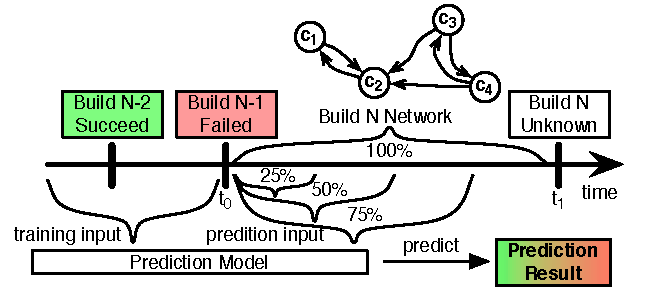
\includegraphics[width=\columnwidth]{figures/ReducedCommunicationInput}
\caption{Predicting Build N Result with different reduced communication
data.}
\label{fig:ReducedCommunicationInput}
\end{center}
\end{figure}

\begin{table}[t]
\small
\begin{center}
%{\small
\begin{tabular}{ r@{\hspace{15pt}}c@{\hspace{5pt}}c@{\hspace{5pt}}c@{\hspace{5pt}}c@{\hspace{5pt}}c@{\hspace{15pt}}c@{\hspace{5pt}}c@{\hspace{5pt}}c}
\toprule
& \multicolumn{5}{ c@{\hspace{15pt}}}{Team Level Builds} &
\multicolumn{3}{c}{Project Level Builds} \\
%\textbf{Naive Bayes} & & & & & & & \\
& B & C & F & P & W & nightly & weekly & beta 	 \\
\midrule
\error\ Recall & .63 & .69 & .62 & .62 & .68 & 1 & .45 & .85 \\ 
\error\ Precision & .43 & .46 & .68 & .75 & .64 & .75 & .83 & .92 \\ 
\ok\ Recall & .60 & .59 & .77 & .80 & .50 & .50 & .75 & .67 \\ 
\ok\ Precision & .77 & .79 & .73 & .69 & .55 & 1 & .33 & .50 \\  
\bottomrule
\end{tabular}
\end{center}
\caption{Recall and precision results only including first 25\% of the
communication.}
\label{tab:Prediction25PResultTable}
\end{table}


Our model can be used by Jazz teams to assess the quality of their current
communication in relation to the result of their upcoming integration. If a team
is currently working on a component and an integration build is planned in the
near future, the measures of the current communication in the team can be
provided as input to our prediction model and the model will predict whether the
build will fail with a precision shown in Table~\ref{tab:PredictionResultTable}.
For example, if team P is working towards a build and our model predicts that the
structure of its current communication leads to a failed build, the team can have
a 76\% (see Table~\ref{tab:PredictionResultTable}) confidence that the build is
going to fail. This information can be used by developers in monitoring their
team communication behavior, or by management in decisions with respect to
adjusting collaborative tools or processes towards improving the integration.

In our analysis we used the complete communication of the build related time
interval as input for the model to predict the build result. In
Figure~\ref{fig:ReducedCommunicationInput}, this is the time interval from $t_0$
to $t_1$ for $Build~N$. This time interval might not be appropriate for practical
applications in which the build process takes only a view minutes, as $t_1$ is
immediately before the build starts. Predicting the build result has no value for
the developers when they have no time left to react on a build failure prediction
and they can simply run the build instead of predicting the result. For long
builds that last several days, the prediction at $t_1$ is still practical
relevant. Developers might delay the build to perform reactive changes on the
failure prediction.

In an additional analysis we investigated the prediction recall and precision by
only considering the communication of reduced time intervals as input for our
model. For each build N result, we trained our model with the complete
communication of all build results except the one from N, and predicted the
result N by only considering the first 25\%, 50\% and 75\% of the communication
as input for the prediction model (see
Figure~\ref{fig:ReducedCommunicationInput}).

We only show the precision and recall of the prediction for the 25\% time range
in Table~\ref{tab:Prediction25PResultTable}, as they are already high enough for
practical use. We observe that the model has almost the same predictive power as
the model considering the complete time range of the build. A possible
explanation is the involvement of work items in many builds. That means that the
task completion time of a work item is longer than the time interval of a build
and task related change sets and communication occurs in multiple builds. When a
developer delivers a change set in the first 25\% of the build related time
interval and the change set is associated to a work item that has already been
discussed, the complete past communication is included. Including the past
communication is valid, as our prediction model learns from the communication
history. In Jazz, a work item is in average included in 5.17 builds (min=1,
median=3, max=57), which provides a possible explanation for having valuable
prediction results even early in the build related time interval.

With the results of this analysis, we are confident that our prediction model is
practically useful, even if it does not consider the complete communication of a
build. Thus, developers and managers have time to react on build failure
predictions before the actual build fails.




\section{Conclusion}
\label{sec:conclusion}
We end this chapter by bringing it back to the initial research questions we set out to answer:
\begin{description}
\item[RQ 1.1] Do Social Networks from repositories influence build success?
\end{description}

The result we presented in Section~\ref{sec:AnalysisResults} show that our predictions, though not highly accurate, outperform random guesses.
Therefore, we conclude that with recall of 55\% to 75\% and precision of 50\% to 76\%, depending on the development team, that communication indeed influences build success.

This finding opens the research avenue of investigating whether the manipulation of communication among software developers can yield positive results with respect to build success.
This leads us to the next research question that we want to search for places within the social networks that we should manipulate to stimulate build success.
For that purpose we turn in the next chapter to the concept of socio-technical congruence that might help us highlighting those developers that should have communicated.

